\documentclass[11pt]{ieeeconf}
\usepackage{graphicx}
\usepackage{float}
\usepackage{lettrine}
\usepackage{caption}
\usepackage{url}


\newcommand\blfootnote[1]{%
  \begingroup
  \renewcommand\thefootnote{}\footnote{#1}%
  \addtocounter{footnote}{-1}%
  \endgroup
}

\title{Bumper Car Sumo}
\author{Jaden Simon - simonjaden223@gmail.com \\ \and
	   Melvin Bosnjak - meco0597@gmail.com \\ \and
	   Daniel Humeniuk - d.humeniuk@utah.edu \\ \and
	   http://bumpercarsumo.weebly.com/}

	   
\begin{document}

\maketitle

\begin{abstract}
Americans are not having fun anymore. The weight of capitalism is forcing families to work 60-hour weeks for low pay, leading to decreased enjoyment and productivity. An affordable and efficient form of entertainment would help solve this issue. In order to promote this, our group is designing a bumper car battle royale game. The project will have intuitive controls, simple yet fun mechanics, and a robust interface to allow for easy development. Continued play testing during development will allow us to monitor these objectives. Our ultimate goal is mutual enjoyment between us and our players.
\end{abstract}

\section{Introduction}
Entertainment is a fundamental part of the human experience. While some lucky few are able to derive satisfaction from their career, most people need something else to entertain themselves. This is the focus of our team's project: to develop an entertaining game with widespread appeal.

 The most important criteria of our game’s success are cost and entertainment efficiency. Our game must yield high levels of fun per minute played, while keeping costs as low as possible without compromising the entertainment value. Competition in games is a key element for high entertainment value \cite{vord:03}.  Because of this, our team decided to create a game where player-controlled robots attempt to push each other out of an arena. To facilitate gameplay, our robots need to be easily pushed around by other robots. Controls should be easy to enhance playability, though not too easy. We need a way to detect game conditions, such as when a robot is out of bounds or when a player wins. This could be done with a human referee, but that would take away immersion of the game. Because some players may not have friends to play with, it is desirable to have an AI to play against. 

Since cost is a contributing factor to our design, we will want to use existing technologies as much as possible. Robots can be constructed as a two-wheeled platform with wireless modules, similar to a Segway. They will be controlled through a web interface accessible by a wide variety of devices. Computer vision libraries will allow us to track the location of each robot if painted differently. Exact positioning solves the problem of detecting game conditions, plus giving us plenty of information to use for a basic AI. 

Our goal, above all else, is that our game is fun. Playtesting will be a major component of our design process, rethinking aspects of the game if it is not fun. Costs will be mitigated, but entertainment value will never be sacrificed for savings. Player enjoyment is our primary measure of success.

% Olliie bot figure
\begin{figure}[H]
\centering
\captionsetup{justification=centering}
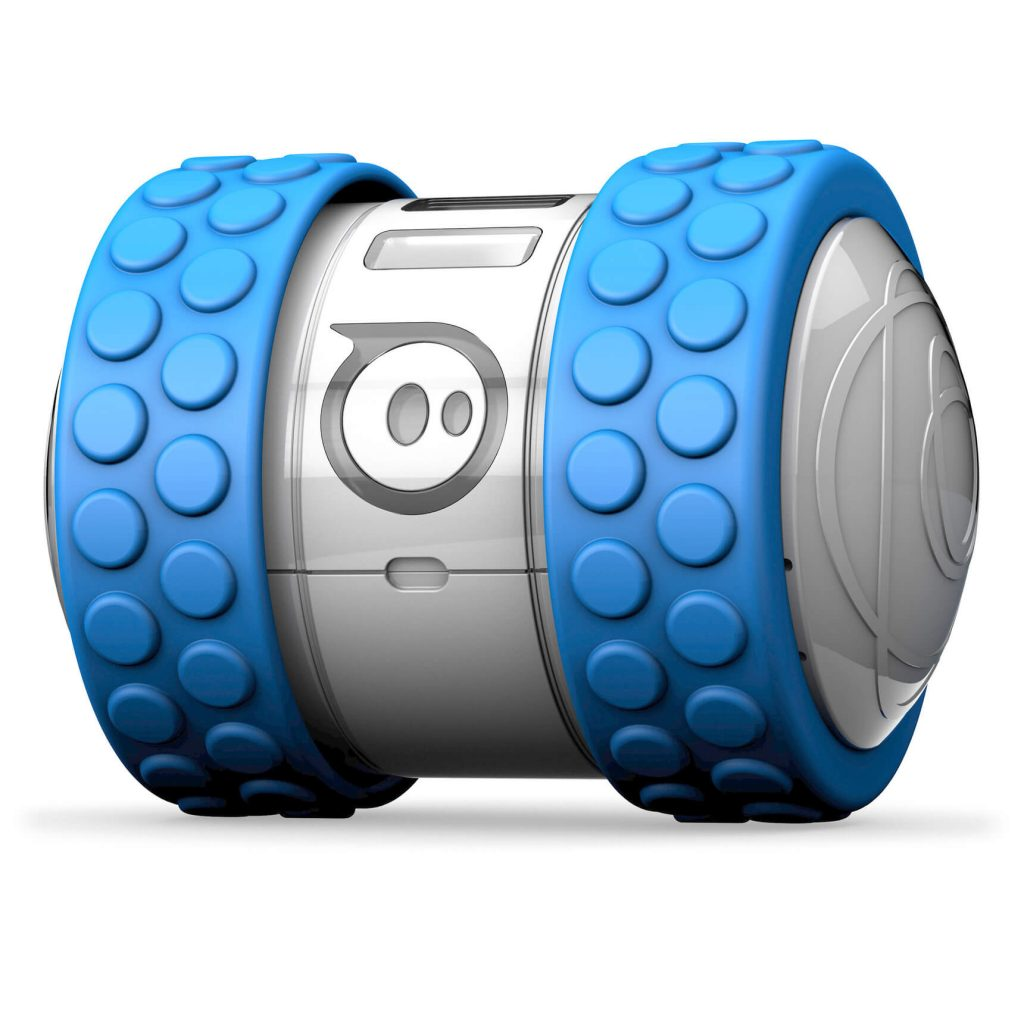
\includegraphics[width=0.5\textwidth]{images/SumoBot.png}
\caption{The Ollie from Sphero\\Source: Adapted from \cite{ollie:19}}
\label{Ollie}
\end{figure}

\section{Background}
The biggest component to our project is the robot. Two-wheeled wireless robots already exist and are mass produced, such as the Ollie (Fig \ref{Ollie}). While the Ollie has many of the features we require for our project, it does not give the level of control necessary to make our game a reality. On top of that, it is expensive at over \$80.00 per unit. The specifications for the Ollie are freely available online and will help guide us through the design of our own robots.


Tracking the robots would be a huge undertaking, but luckily there exists an open-source computer vision library called OpenCV. OpenCV provides algorithms to scan an image and identify desired patterns \cite{opencv:19}. With this, tracking can be done with only a camera, a computer, and a small bit of code. 

\section{Design}

To complete the project, we will need a main control mechanism (a hub), robots, controllers, and tracking. A centralized hub will be the core of the project, which will coordinate the other three components. The robots will use a custom PCB with an inertial measurement unit (IMU) and low-voltage motor driver, able to communicate via WiFi through an ESP8266. Our controllers will have both a physical and software interface. An overhead camera will be used to monitor the locations of our robots, which will be combined with IMU data for an extremely accurate positioning system. Separating these four components allows for simultaneous development by our team members.

\subsection{Hub}
The hub will be a Raspberry Pi device that will have a few functions:
It will capture the game state from a camera peripheral. The camera will be hooked directly into the Raspberry Pi and the hub software will have to continuously take the frame data from the camera and pass it as an input to openCV. The hub software will then associate the color of the robot with the location openCV outputs to keep track of each robots location. This process will be on its own thread that will have to share memory with the thread that is running the game loop. This allows the game logic to know the location of robots at all times. This means we will have to eliminate race conditions with thread locks. A flowchart is shown in \ref{flowchart}.

Another thread will be hosting a server. The server will have communication with the controllers, and each robot. This thread will be a loop that takes in player inputs, updates the game state, then sends the appropriate commands to the robots. The hub will most likely have to hold many game models to support the game modes.

Fig. \ref{Illustration} shows the basic illustration of the game. If time allows, then our AI implementation will be done on the hub. This component of the project requires no custom hardware and can be done entirely in software. The Core hub software will take at most a month for full development and testing. 

% Game design figure
 \begin{figure*}[!t]
  \centering
  \captionsetup{justification=centering}
      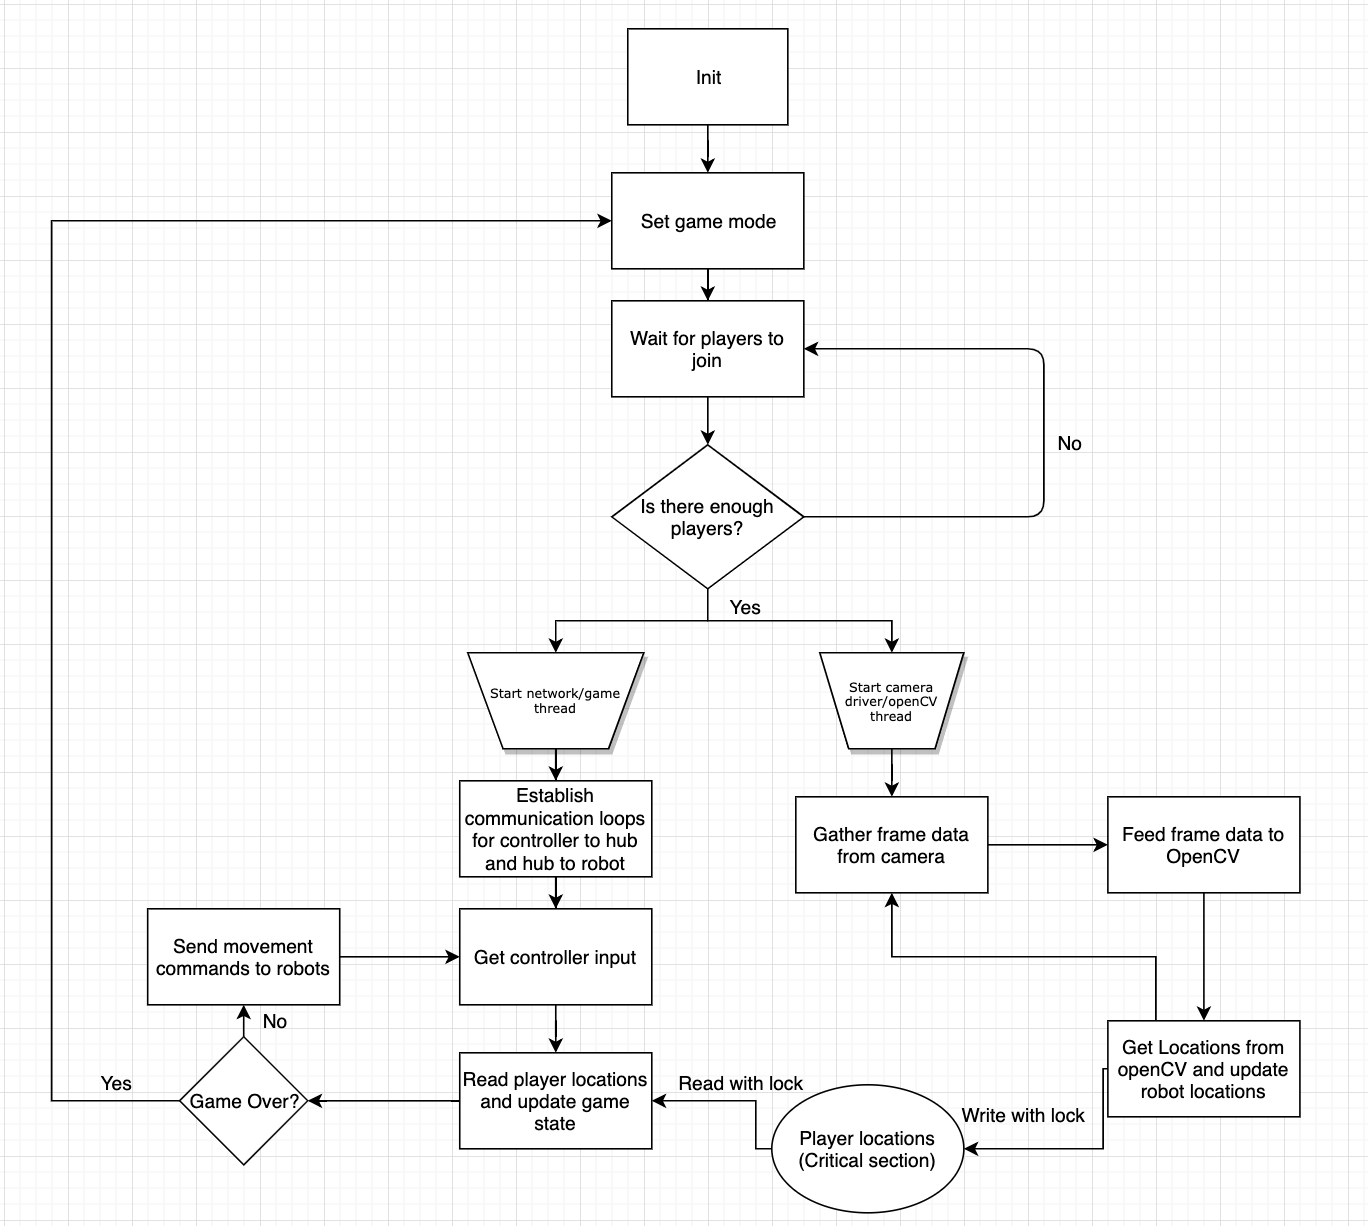
\includegraphics[width=14cm]{Initial Proposal for Senior Project/images/Flowchart.png}
        \caption{Overall game design}
        \label{Illustration}
\end{figure*}



\subsection{Robot}
% Describe in more detail 

Our robots will be cylindrically shaped with two wheels on each side of the body that can move in either direction (Fig. \ref{RobotFig}). In order to move forward, both of the wheels will spin at the same time at the same rate. To move backwards, the same principle applies in the opposite direction. Rotating the robot left or right requires spinning the motors in opposite directions. An ESP8266 microcontroller will provide WiFi and Bluetooth capability while also allowing for command interpretation from the hub. Our motors will require significant current so a custom driver will be required. The torque of our motors is important for our robots to be able to push each other around. Additional components can be added to keep track of orientation or acceleration. Batteries of suitable capacity and voltage will be determined once the robot requirements are finalized. The robot will take up to 3 months to fully develop and test due to its requirement of custom hardware. 

% Robot design figure
 \begin{figure}[H]
  \centering
      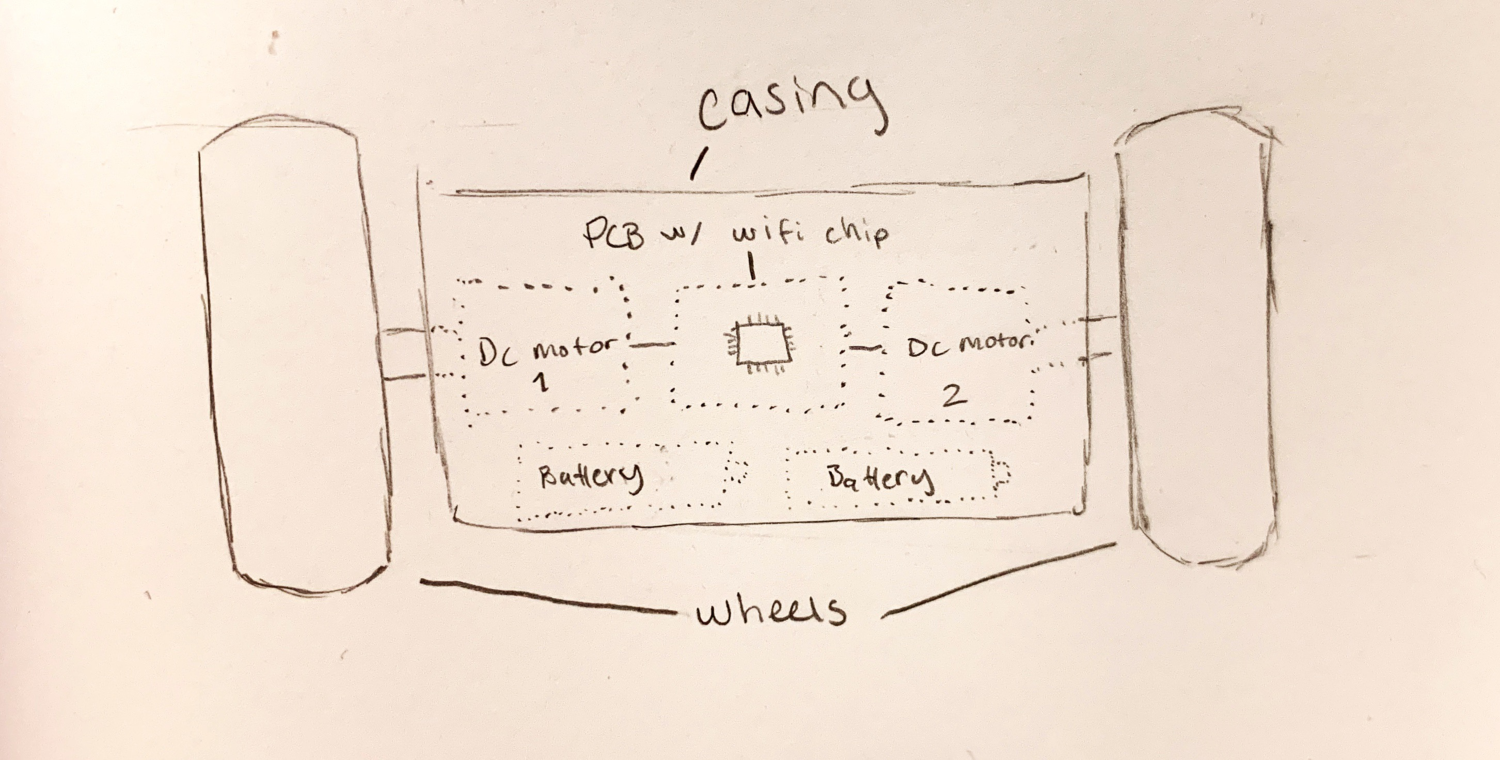
\includegraphics[width=0.5\textwidth]{images/RobotSketch.pdf}
        \caption{Basic robot layout}
        \label{RobotFig}
\end{figure}

\subsection{Controller}
% Talk about using Wii balance board and/or game console controller 
% Maybe talk about other ways to control the robots ? 

The controller provides the opportunity to add interesting game mechanisms that are unique to our game. We have been discussing ideas for unique control options and have come up with several ideas. We are developing and interfacing multiple controllers to give players a choice in their play style as well as providing backup plans if one or more turn out to be unenjoyable. The ideas we are pursuing are utilizing a web server, Wii Balance Board, and Nintendo controllers. The web server involves players logging into a website and using keyboard inputs to move the robots as they watch the game through the web camera. The Wii Balance board, as seen in Fig \ref{Wii}, allows for a more interesting and challenging style of play by utilizing player movement. The Nintendo controllers will include Super Nintendo and Nintendo 64 controllers that will plug directly into the Raspberry Pi Hub. Each controller will be discussed in further detail below with their respective priority level.

% Wii fit board figure
\begin{figure}[H]
\centering
\captionsetup{justification=centering}
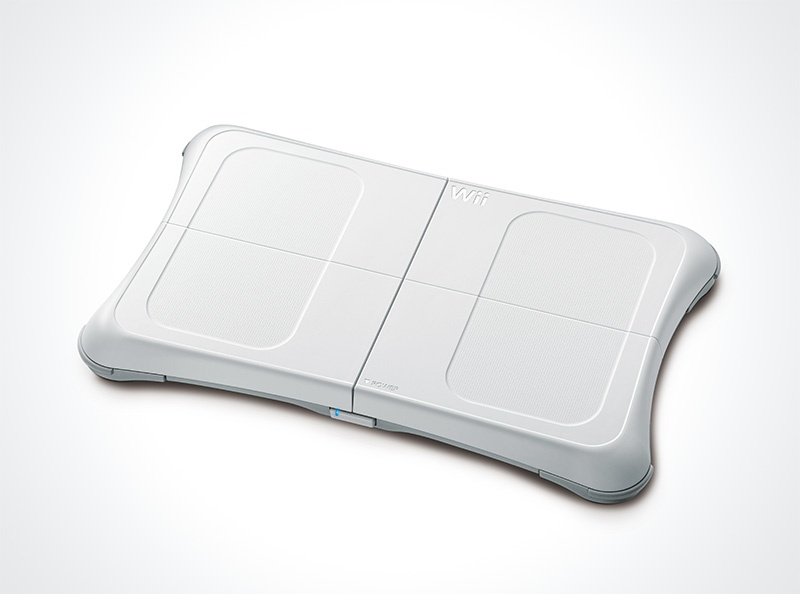
\includegraphics[width=0.5\textwidth]{images/wii.jpg}
\caption{The Wii Balance Board may be an ideal candidate for a unique control system \cite{wiiboard:19}}
\label{Wii}
\end{figure}

A web-based control system is currently the cheapest controller option with some possibilities to enhance the playing experience. The users will need to use their personal WiFi enabled laptops to log into a website we will develop for the game and select a robot to play as. The website will be streaming a live feed of the game play area via the web camera that will also be handling the tracking capabilities. The players will receive a brief overview of the controls that are enabled on their keyboards and are then allowed to select the robot of their choice. Once a robot is selected, any physical controller in the game area will be disabled. The robots will be driven forward, back, left, and right with the use of key presses. The key presses will be sent to the Hub which will process the information and pass it on to the respective robot. We will work on limiting latency between button presses and movement of the robot. This controller will be medium priority as the implementation will be more of a challenge than the Wii Fit Board but it is simple enough to not require a large allocation of our time.

If time allows, we will make further use of OpenCV and add extra features to the web interface. The robots will be tracked on screen with and player names will be displayed above their respective robot. This also adds potential to enhance the game with power-ups for certain game modes. We will also enhance the controller by adding graphics and notifications when games are won, lost, begin, and end. The added features will add to the appeal to this controller.

The Wii Balance Board promises an interesting controller experience. We will interface with the board to receive output from standard user inputs to the board. From there, we can interpret the data in the control hub. There are many references online that will assist in interfacing with the controller. The Wii Balance Board uses a Bluetooth profile called Human Interface Device Profile which we will need to interface with and interpret the data as we need. As seen in \cite{homebrew}, the Wii Balance Board uses 16-bit pressure sensors. With four sensors total, it will be possible to enable two sensors to assist in driving one motor. Once the device has been interfaced with, we will collect input from the device by standing on it and leaning forward, back, left, and right. Once we can see what the average output will be for these measurements, we can effectively write the software for the Hub to interpret the data to drive the robot. The board feature will provide users with both interesting and challenging gameplay. This controller requires the highest priority as it will take time to ensure we are interfacing properly with the board's Bluetooth profile. 

There are many variations of Nintendo controllers currently available online that will be the fastest controller option to implement. The authors of \cite{controller:19} inform us that no additional drivers are needed for many of the available controllers which will ease the process of interfacing them with the Hub. Fig \ref{Controllers} shows a Super Nintendo controller on the right and a Nintendo 64 controller on the left. The Super Nintendo controller has a simple D-pad to steer the robots which will makes the directional input easier to interpret and the extra buttons will be used for speed control. The Nintendo 64 controller has a D-pad for steering as well as a joystick. We can use the joystick to control the speed and direction of the robot. The Hub will account for both types of steering depending on which controller is being used. This controller remains at the lowest priority as the interfacing has already been done. The biggest task with these controllers is to interpret their output data and relay the result to the robots.

% USB controllers
\begin{figure}[H]
\centering
\captionsetup{justification=centering}
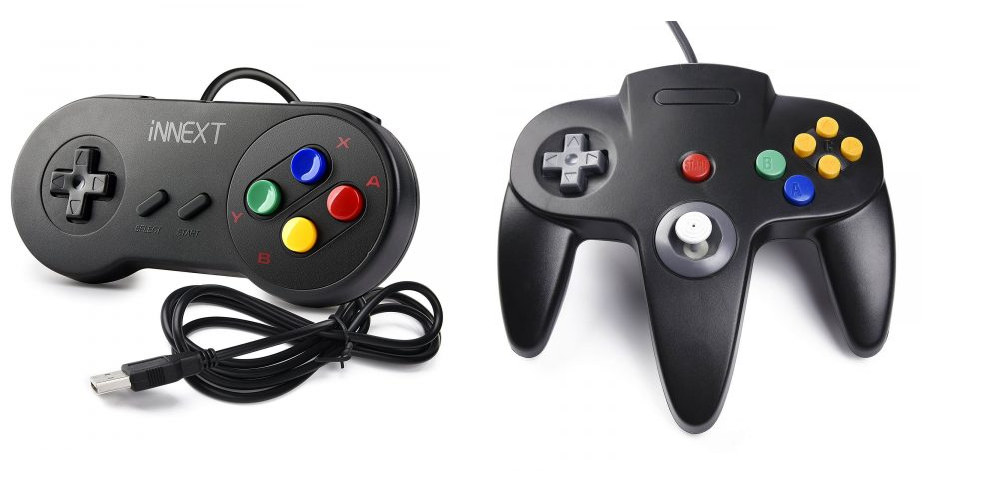
\includegraphics[width=0.5\textwidth]{images/controllers.png}
\caption{Two USB controller options \cite{controller:19}}
\label{Controllers}
\end{figure}

While electing to use Nintendo controllers is not the most original option, this is the option that we are the most confident in as a backup plan. The USB allows for a fast and painless implementation. There is also benefits to the players having familiarity with game paddles which will allow them to enjoy the ease in controlling the robots. We can also add interesting ideas during the play-testing phase of the project. Once all required components of the game are complete, features will be added that utilize the extra buttons on the Nintendo controllers. With the Nintendo controllers, we are safe to explore other controller options such as the web server and Wii Fit Board and know that the Nintendo controllers will be an viable fallback. 

The choice to implement multiple controllers provide more options for the players and gives us more possibilities to explore our creativity. This also gives room for us to continue adding controllers that can be implemented with extra game modes offered, similar to the business model of Downloadable Content (DLC) that is featured in most modern video games. The controllers have been selected to provide the users with a new and challenging experience and will be modified and added to until they provide that experience. 

\subsection{Tracking}

Tracking will be done by the hub using a camera and OpenCV. The casings for each robot will be designed in such a way to allow for easy identification by algorithms. Players who leave the camera's field of view will be considered eliminated by the hub, preventing control of the robot by the player. Since our camera will be static, the total play area is limited by our camera's height and field of view. Our play surface will be monochromatic which increases our tracking capability, though we should be able to track with an arbitrary surface. The timeline for tracking is largely dependent on the hub and the robot, though 2 weeks seems like a reasonable amount of time.

\section{Game Mechanics}

\subsection{Game Modes}

There will be many game modes to select from. The primarily plan was to design the game arena to accommodate only one game mode. The team has elected to enable for multiple game modes to provide longevity to the product.    

\section{Timeline}
In order to finish our project before demo day, we have created a timeline. While the deadlines listed here are not set in stone, it should give us a good idea of what we need done by when. The length of the bars represent about how long it should take to complete the task. Each group member is assigned to a certain task dependent on the bar's color, though there is some flexibility there as well. Some of the tasks are dependent on the completion of previous tasks, so it is important for us not to get too far behind schedule. 

\subsection{Spring}
For the remaining month of May we will finalize our required parts list. This includes verifying we have the correct parts, checking availability, and price calculations.

\subsection{Summer}
The summer will consist of ordering and gathering the resources needed as well as detailed design for each component of the project. Basic documentation of our hardware and software interfaces will be completed by the end of the summer. We will complete a basic software interface and start experimenting with hardware interfaces. If time allows then we can create a basic play surface, since it is not dependent on the completion of any singular component.

\subsection{Fall}
Most of the legwork for the project will be done during the fall. With all components gathered and the design completed all that will be left to do is to assemble, test, and finalize documentation. Each project component will be worked on simultaneously. Integration between the four components of the project will not take long if our interfaces were designed correctly, perhaps only a week or two. The minimum requirements of the project is planned to be completed and tested a month before the demo day. A large amount of extra time allows us to experiment with additional features that will hopefully add to the entertainment value.

\subsection{Component Assignments}
As already discussed, the project is separated into 4 key components. Each component will have a single group member act as lead developer. Robots and tracking will be managed by Jaden. Development of the hub and its communication protocol will be done by Melvin. Dan is tasked with creating the software controller interface as well as working on variations of hardware interfaces. 


\section{Milestones}
% Every person needs at least 5 milestones 
Each group member will have at least 5 milestones to their assigned component: 

\subsection{Melvin}
For Melvin, his component will be heavily involved with the Hub device, so the first milestone will be getting a basic network connection with multiple ESP8266 client devices. This will be done over the summer. This should be quick as we have demonstrated working a client server network connection for the prototype. During Demo day this will be shown with the ability to control each robot wirelessly as this will require handling multiple wireless connections simultaneously.

The second milestone will be creating a communication API with the Hub. This will consist of designing a protocol to support controller to hub commands and hub to client commands. This will be tested once we test connecting the whole system together. This will also be shown with the ability to control each robot wirelessly. This will also be done this summer.

The third milestone will be to interface the hub device with the camera peripheral that we will use to capture the game state. This will include ordering the appropriate camera for our tasks, figuring out how to gather frame data from the camera, and propagating that frame data to OpenCV. This will be shown by the ability to detect when a robot has gone out of the play area. This will be done later in the summer.

The fourth milestone will be to create a model that captures and processes the game state within the hub so that it can easily control game mechanics. This will have to continuously read the game state from the camera API and store it in its internal model. Based on the model, it will then send the appropriate commands/data to clients. This will be made very modular in order to support multiple game modes. This will be done in the fall along with the last milestone. This will be shown by the hubs ability to manage a game and keep track of score, winner etc.

The last milestone will be to integrate and test the hub with the whole system. This will depend on the state of each other component, but we would like to leave at least a month before demo day to complete this milestone in order to leave time for integrating stretch goals and finalizing the project. This will be shown by the system working as expected.

\subsection{Jaden}

\subsection{Dan}

\section{Resources}
% Flesh out this section (full BOM) 
% Part number, lead time, unit cost, quantity, form factor, etc.
\subsection{Bill of Materials}

Each robot will require 2 DC motors with wheels, several batteries, a PCB that includes an ESP8266 microcontroller and motor drivers for each DC motor, and a casing to enclose and protect the internals. The casing will be designed and 3d printed by our group. Various ICs and small electrical components will be required based off our circuit designs. The design, testing, and implementation of the robot will take the bulk of the time required for this project.

A Raspberry Pi will act as the hub, handling all game mechanics and user-robot interactions. The Raspberry Pi 3 Model B+ has a quad core 1.4GHz processor which should be enough processing power for these tasks. Tracking is a fundamental component of the hub and will require a camera, ideally with high resolution and FPS. The options for the camera are the Raspberry Pi camera and the Logitech C922x Pro Stream Webcam. Software on the hub will depend on multiple open source libraries to function, though will still require significant custom software to operate.

The playing field will be constructed out of a simple table top with some 2 x 4's to hoist up the camera, with power and data cables running down to connect to the hub.

\subsection{Vendor List}
% List all vendors with contact information 

\section{Group Logistics}
In order to stay on top of our set deadlines, our group will be meeting at least once a week to discuss current tasks, issues we have experienced, and new ideas for our game. These meetings are logged on our website. Because Melvin will be in Idaho for the duration of the summer, our meetings will have to be digital and infrequent. In the fall we will resume the weekly meetings.

\section{Risk Management}
% Describe risks for each task, some might not have any
For the Hub device, Some potential risks with this is latency, and computing power. The Hub device has many responsibilities such as camera I/O, game logic, handling many network communication channels, and running OpenCV. In order to reduce these risks the Hub will be using UDP connections with each client and multi-threading each task. This will also be done over the summer. This will require a device that has multiple cores, wifi capabilities, and a fast processor. That is why we chose the Raspberry Pi 3 Model B+.

\section{Testing}
Much of our time spent testing will be focused on robot design and user experience. The most complicated part of our robot will be the integration of a battery, but once that is complete we will focus on debugging software communication protocols. In addition, play-testing of the project is fundamental to our success. We must ensure that our game is entertaining through repeated testing of robot collisions and the user interface. Collisions with robots should feel powerful and the user interface should be responsive and free of frustration. Beyond that, we will need to experiment with the durability of our robots to make sure they do not break during play.

\section{Project Demo}
% Describe what will be highlighted in the demo 

On demo day, we hope to achieve a minimum requirement of 4 robots, basic user interface, and a single game mode. While 4 robots will provide enough competition to be entertaining, we ideally want 8 robots to allow more people to play. Basic user interface would only have options to control the robots in the 4 cardinal directions. More game modes are simple to implement but add enormous entertainment value.

\subsection{Setup}
First players connect to our web server through a device of their choice. Connections made in previous rounds will be preserved. Players then choose an available robot to play as. Each selected robot must be placed in designated spots, which will have to be done by humans. Once the hub detects that all robots are in the play area, the game can begin. 

\subsection{Game Round}
Each game round will depend on the game mode. In all of our game modes, players are eliminated if their robot leaves the play area. For a free-for-all, the game round ends when all but one player is eliminated. If a team mode is implemented, then a game round ends when only a single team remains. Game modes may have time limits, though this will depend on play testing during development.

\subsection{Post Game}
If we are able to meet our minimum requirements, then additional features will be added to aid user experience. This would include post game reports that contain information about the player such as eliminations, maximum speed, or the biggest hit taken. After any post game reports, our demo will start again at the setup.

\section{Project Status}
% Current status of our project
% Robot PCB pretty much
The current status of our project largely comes from our prototype. We have demonstrated wireless communication in a client server architecture. We have also gotten the first version of our robot PCB fabricated and tested which had some problems, however, we have learned from the first version which will make for a much more robust second version. 

\section{Conclusion}
% Summarize entire proposal, include lessons learned so far (management/team/engineering) 
% Include biggest risks, analyze task dependency 
% Final advertisement of project 

\bibliographystyle{IEEEtran}
\bibliography{IEEEabrv,bib/ref}

\end{document}